%=============================================================================
% chktex-file 1 chktex-file 8 chktex-file 12 chktex-file 13 chktex-file 24 chktex-file 26
% CHAPITRE 4 : RÉALISATION ET IMPLÉMENTATION
%=============================================================================

\chapter{Réalisation, Pipeline IA et Validation}
\label{chap:realisation}

\section{Introduction}

Ce quatrième chapitre détaille la concrétisation logicielle de la plateforme \textbf{\projectShortTitle}. Nous présentons d'abord l'environnement de développement et de déploiement, puis nous détaillons le fonctionnement du pipeline d'intelligence artificielle dédié à l'analyse des rapports d'expertise. Nous exposons ensuite les principales interfaces utilisateurs conçues, avant de conclure par la méthodologie de test et les résultats de la validation expérimentale.

\section{Environnement Technologique et Outils de Développement}

La réalisation du projet s'appuie sur une pile logicielle moderne et complémentaire, résumée dans le tableau~\ref{tab:tech_stack}.

\begin{table}[H]
\centering
\small
\caption{Synthèse de la pile technologique de la plateforme LeasRecover}
\label{tab:tech_stack}
\begin{tabularx}{\textwidth}{@{}L{3.5cm} L{3.5cm} Y@{}}
\toprule
\textbf{Couche / Domaine} & \textbf{Technologie} & \textbf{Rôle et Justification} \\
\midrule
\textbf{Interface Utilisateur} & Next.js 16 (React, TypeScript) & Rendu hybride rapide, typage statique strict et intégration de la bibliothèque Ant Design. \\
\addlinespace
\textbf{Couche BFF (Sécurité)} & Node.js / Next.js Server & Gestion sécurisée des sessions par cookies chiffrés \code{HttpOnly} sans exposition de tokens. \\
\addlinespace
\textbf{Noyau Métier Backend} & Spring Boot 4 (Java 21) & Gestion transactionnelle robuste, moteur de workflow et routage dynamique multi-tenant. \\
\addlinespace
\textbf{Service IA \& NLP} & FastAPI (Python 3.11+) & Microservice asynchrone pour le traitement documentaire, PyMuPDF et modèles LLM. \\
\addlinespace
\textbf{Persistance} & PostgreSQL 18 & Base de données relationnelle avec schémas séparés par tenant et intégrité ACID. \\
\addlinespace
\textbf{Conteneurisation} & Docker \& Docker Compose & Orchestration unifiée garantissant l'isolation des microservices et la portabilité. \\
\bottomrule
\end{tabularx}
\end{table}

\section{Implémentation du Pipeline IA}

\subsection{Architecture du Pipeline Asynchrone}

L'ingestion et l'analyse d'un rapport d'expertise PDF non structuré s'exécutent selon une chaîne de traitement asynchrone représentée dans la figure~\ref{fig:pipeline_ia}.

\begin{figure}[H]
\centering
\begin{tikzpicture}[
    scale=0.78, every node/.style={transform shape},
    node distance=1.2cm and 1.4cm,
    stepbox/.style={
        rectangle, draw=primaryblue, fill=lightgrey, line width=1.1pt, rounded corners=5pt,
        minimum width=2.8cm, minimum height=1.3cm, align=center, font=\sffamily\small, drop shadow
    },
    flowarrow/.style={
        -{Stealth[scale=1.1]}, line width=1.3pt, color=secondaryblue
    }
]

% Nodes
\node[stepbox, fill=accentorange!15] (docIn) {\textbf{Ingestion}\\[2pt]Rapport PDF\\(Scan / Vecteur)};
\node[stepbox, fill=primaryblue!15, right=of docIn] (preproc) {\textbf{Prétraitement}\\[2pt]Extraction PyMuPDF\\\& Binarisation};
\node[stepbox, fill=secondaryblue!15, right=of preproc] (extract) {\textbf{Extraction Sémantique}\\[2pt]NLP / LLM Parsing\\\& Regex Montants};
\node[stepbox, fill=accentgreen!15, right=of extract] (decision) {\textbf{Rapprochement}\\[2pt]Calcul $\Delta = \ve - \vr$\\Indicateur Tripartite};

% Connections
\draw[flowarrow] (docIn) -- (preproc);
\draw[flowarrow] (preproc) -- (extract);
\draw[flowarrow] (extract) -- (decision);

\end{tikzpicture}
\caption{Pipeline d'ingestion et d'extraction IA des rapports d'expertise}
\label{fig:pipeline_ia}
\end{figure}

\subsection{Algorithme d'Extraction et de Confrontation Financière}

L'algorithme~\ref{alg:extraction_ia} résume le processus d'analyse documentaire, d'extraction des métriques clés (valeur vénale estimée $\ve$, kilométrage, frais de remise en état) et de calcul du score de fiabilité.

\begin{algorithm}[H]
\caption{Algorithme d'extraction et de validation des données d'expertise}
\label{alg:extraction_ia}
\begin{algorithmic}[1]
\REQUIRE Document PDF $D$, Valeur résiduelle contractuelle $\vr$
\ENSURE Tuple $(\ve, \text{Kilométrage}, \Delta, \text{Fiabilité}, \text{ScoreConfiance})$
\STATE $\text{TexteBrut} \leftarrow \text{PyMuPDF\_Extract}(D)$
\IF{$\text{Longueur}(\text{TexteBrut}) < 50$}
    \STATE $\text{TexteBrut} \leftarrow \text{OCR\_Fallback}(D)$
\ENDIF
\STATE $\ve \leftarrow \text{ExtraireEntitéFinancière}(\text{TexteBrut}, \text{cible}=\text{« valeur »})$
\STATE $\text{Km} \leftarrow \text{ExtraireEntier}(\text{TexteBrut}, \text{cible}=\text{« kilométrage »})$
\STATE $\text{Frais} \leftarrow \text{ExtraireMontant}(\text{TexteBrut}, \text{cible}=\text{« frais »})$
\STATE $\text{ScoreConfiance} \leftarrow \text{CalculerScore}(\ve, \text{Km}, \text{TexteBrut})$
\STATE $\Delta \leftarrow \ve - \vr$
\STATE $\text{Ratio} \leftarrow (\ve / \vr) \times 100\%$
\IF{$\text{Ratio} \ge 100\%$}
    \STATE $\text{Fiabilité} \leftarrow \text{« Favorable (Vert) »}$
\ELSIF{$\text{Ratio} \ge 75\%$}
    \STATE $\text{Fiabilité} \leftarrow \text{« Écart Modéré (Orange) »}$
\ELSE
    \STATE $\text{Fiabilité} \leftarrow \text{« Écart Critique (Rouge) »}$
\ENDIF
\RETURN $(\ve, \text{Km}, \Delta, \text{Fiabilité}, \text{ScoreConfiance})$
\end{algorithmic}
\end{algorithm}

\section{Présentation des Interfaces Utilisateurs}
\label{sec:interfaces}

L'ergonomie et le design de la plateforme \textbf{\projectShortTitle} ont été spécifiquement conçus pour répondre aux exigences des gestionnaires de recouvrement et des analystes financiers en contexte institutionnel. L'interface privilégie une hiérarchisation stricte de l'information (\textit{Urgency First}), une réduction maximale de la charge cognitive et une transparence décisionnelle totale. Cette section détaille les écrans majeurs développés pour la solution.

%------------------------------------------------------------------------------
\subsection{Écran d'Authentification et Contrôle d'Accès Sécurisé}
\label{subsec:screen_login}

L'écran de connexion (Figure~\ref{fig:screen_login}) constitue le point d'entrée unique de la plateforme pour deux populations distinctes grâce à un sélecteur segmenté (\textit{Société (Tenant)} / \textit{Super Administration}) :
\begin{itemize}
    \item \textbf{Espace Société :} Le gestionnaire saisit l'identifiant unique de son organisation (\code{Tenant UUID}), son adresse électronique et son mot de passe.
    \item \textbf{Super Administration :} Dédié aux administrateurs de la plateforme pour le provisioning des sociétés de leasing partenaires, sans accès aux données confidentielles des dossiers.
\end{itemize}

Sur le plan technique et sécuritaire, cette interface s'appuie sur le modèle \acro{BFF}{Backend-for-Frontend} de Next.js. Lors de la validation des identifiants, un cookie chiffré \code{HttpOnly} et \code{SameSite=Strict} est injecté dans le navigateur de l'utilisateur. Aucun jeton sensible (JWT) n'est stocké dans le \code{localStorage}, immunisant ainsi l'application contre les attaques de type \acro{XSS}{Cross-Site Scripting}.

\begin{figure}[H]
\centering
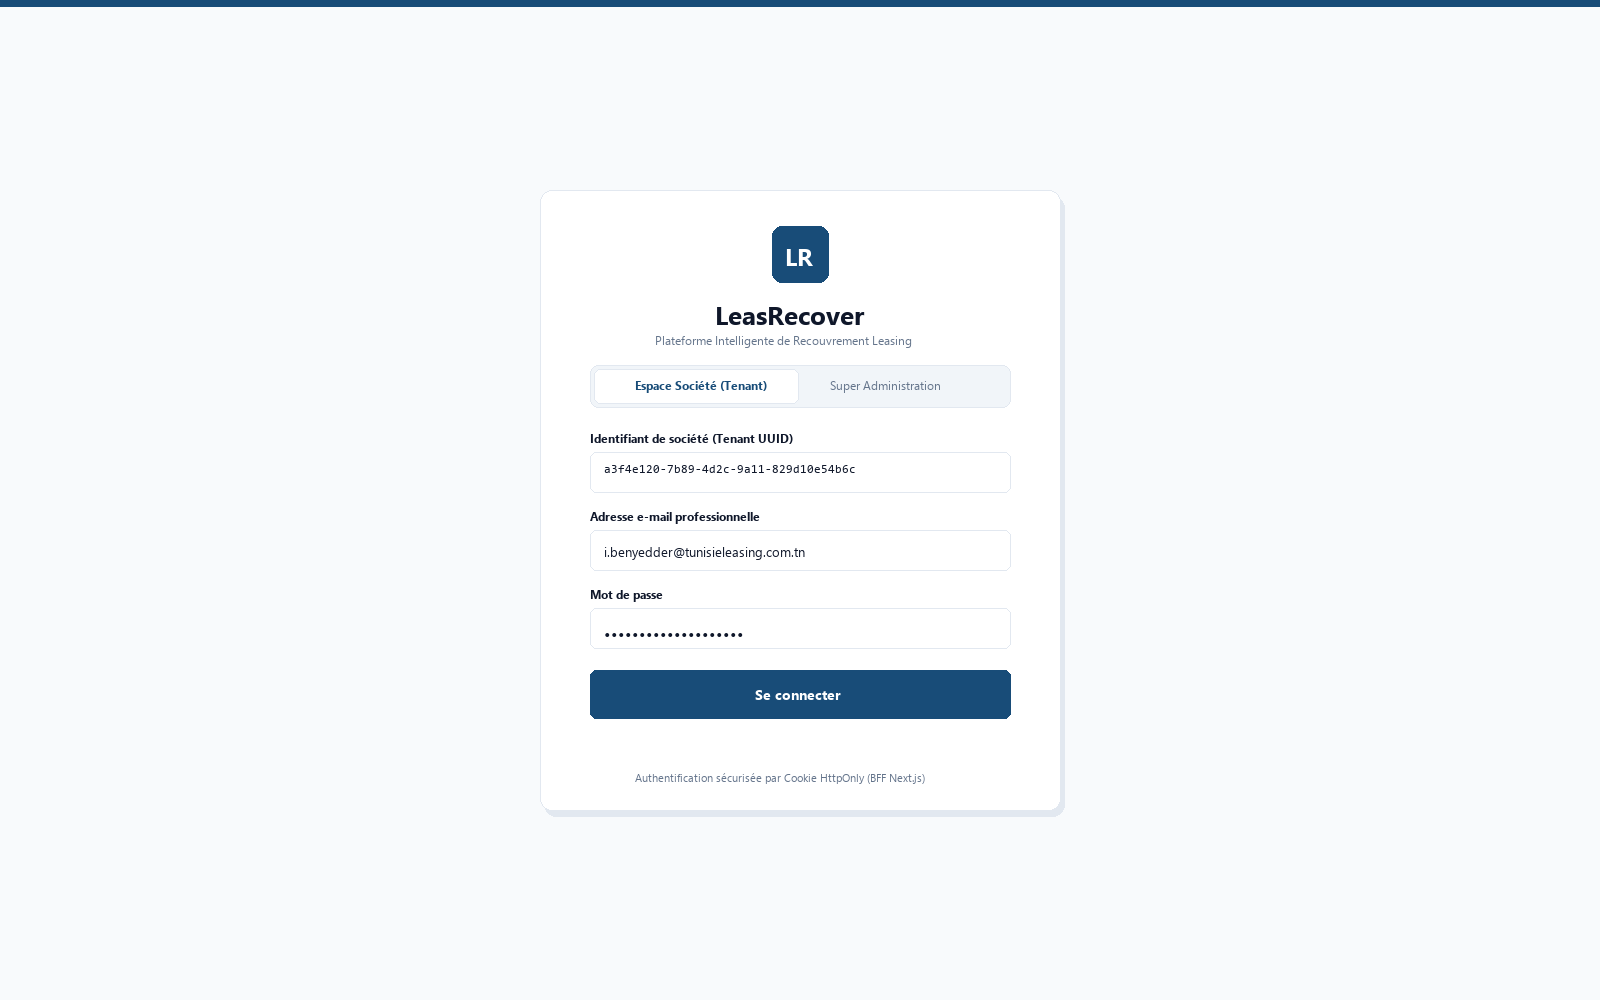
\includegraphics[width=0.92\textwidth,keepaspectratio]{images/screen_login.png}
\caption{Écran d'authentification sécurisée multi-tenant avec isolation BFF}
\label{fig:screen_login}
\end{figure}

%------------------------------------------------------------------------------
\subsection{Tableau de Bord de Pilotage et Registre des Dossiers (Command Center)}
\label{subsec:screen_dashboard}

Le tableau de bord (Figure~\ref{fig:screen_dashboard}) représente le centre névralgique du gestionnaire de recouvrement. Il centralise la totalité du portefeuille de contentieux et hiérarchise immédiatement les urgences opérationnelles :
\begin{itemize}
    \item \textbf{Indicateurs de Synthèse (KPIs) :} Visualisation en temps réel du nombre total de dossiers actifs (62 dossiers), du montant global des valeurs résiduelles en risque (2\,840\,500~TND), des échéances légales imminentes et du taux d'automatisation des arbitrages IA (94.8\,\%).
    \item \textbf{Flux d'Alertes Prioritaires :} Bandeau dynamique situé au sommet de la page, mettant en exergue les dossiers nécessitant une intervention urgente (délais légaux sous 48h, dormance critique de dossiers sans action depuis plus de 21 jours). Chaque alerte offre un bouton d'action contextuel permettant de sauter directement à l'étape requise.
    \item \textbf{Barre de Recherche et Filtrage à Facettes :} Recherche textuelle instantanée (client, référence, immatriculation) et filtres combinables par phase de recouvrement, statut et fiabilité de l'expertise IA.
    \item \textbf{Registre Tabulaire Paginé :} Tableau à haute densité d'information présentant l'état d'avancement, le gestionnaire affecté, la valeur résiduelle et le badge de fiabilité issu du pipeline IA.
\end{itemize}

\begin{figure}[H]
\centering
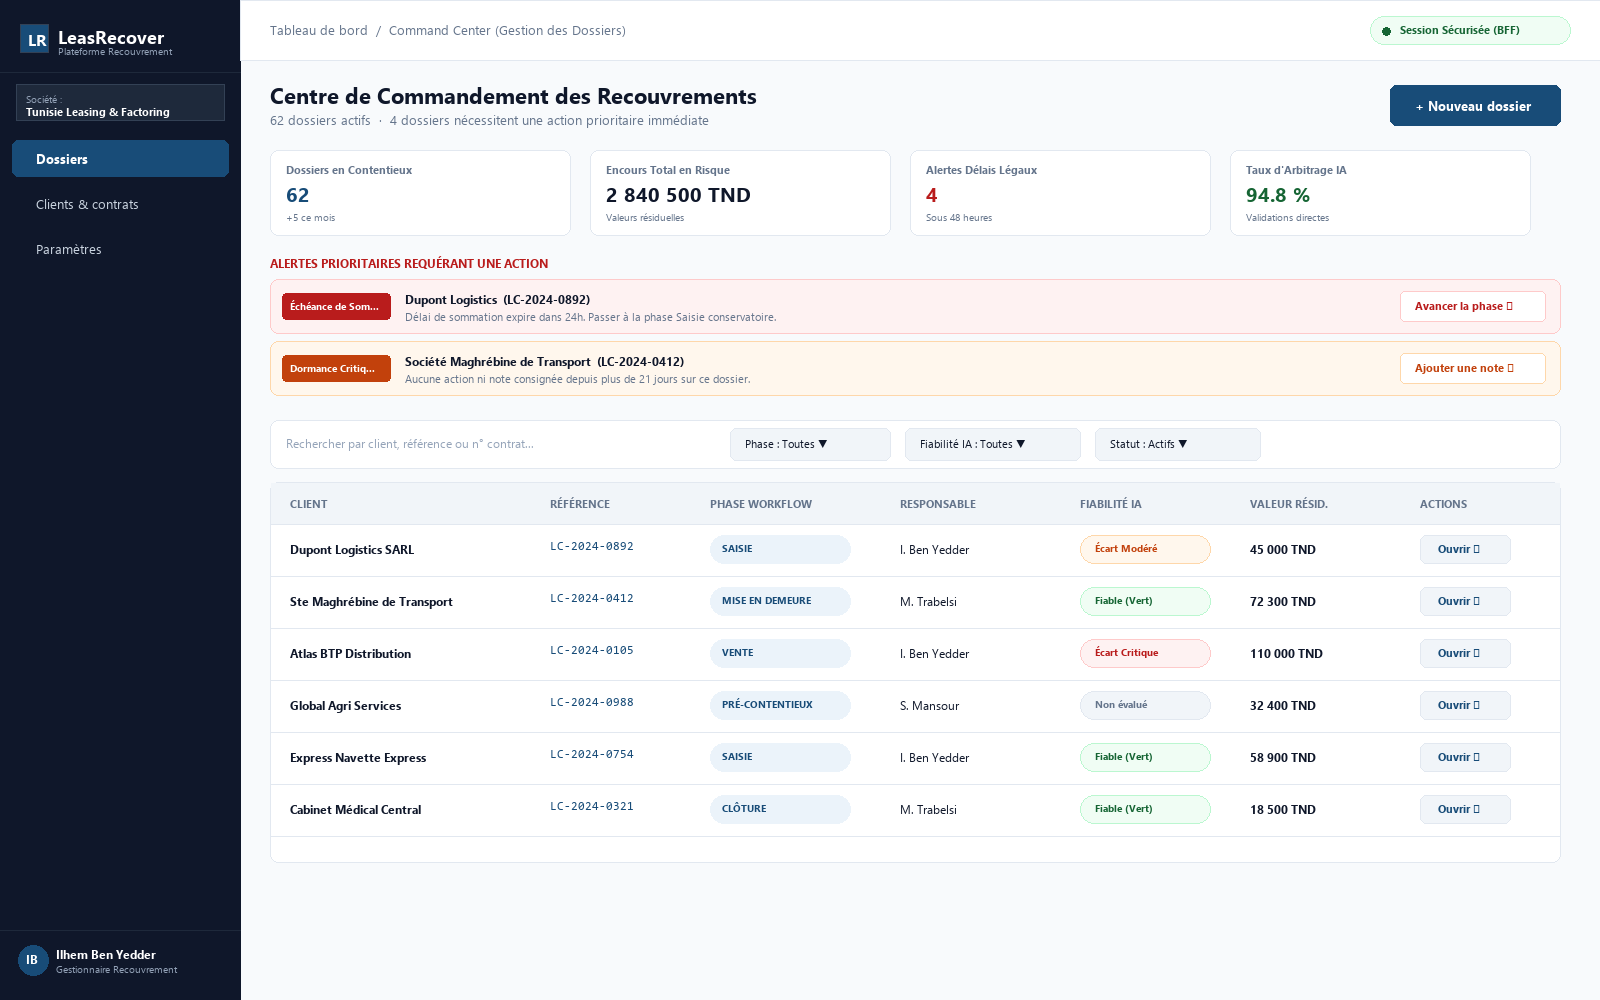
\includegraphics[width=0.95\textwidth,keepaspectratio]{images/screen_dashboard.png}
\caption{Centre de commandement (\textit{Command Center}) et flux d'alertes proactives}
\label{fig:screen_dashboard}
\end{figure}

%------------------------------------------------------------------------------
\subsection{Fiche Dossier Interactive et Moteur de Workflow Métier}
\label{subsec:screen_case_detail}

La vue détaillée d'un dossier de recouvrement (Figure~\ref{fig:screen_case_detail}) orchestre le cycle de vie complet du contentieux autour des cinq phases juridiques obligatoires :
\begin{itemize}
    \item \textbf{Barre de Progression Interactive (\textit{Phase Stepper}) :} Positionne visuellement le dossier au sein des cinq jalons (\textit{1. Pré-contentieux}, \textit{2. Mise en demeure}, \textit{3. Saisie}, \textit{4. Vente}, \textit{5. Clôture}). Les étapes validées sont marquées en vert, la phase courante en bleu primaire, et les étapes futures sous cadenas.
    \item \textbf{Gestion des Prérequis et Verrous Bloquants :} Le moteur de règles évalue dynamiquement les conditions nécessaires pour franchir une étape. En cas d'incomplétude (par exemple, absence du rapport d'expertise ou de l'ordonnance de saisie), une bannière explicite indique précisément la pièce manquante et désactive l'avancement.
    \item \textbf{Volet Latéral Persistant (\textit{Sticky Aside}) :} Synthétise les informations financières fondamentales (valeur résiduelle contractuelle, valeur d'expertise estimée, écart $\Delta$, gestionnaire responsable et prochaine échéance légale).
    \item \textbf{Espace Multi-Onglets :} Permet de naviguer sans rechargement de page entre les détails contractuels du débiteur, les caractéristiques du véhicule gagé, le journal des notes collaboratives, l'historique d'audit immuable (technologie Hibernate Envers) et la gestion documentaire.
\end{itemize}

\begin{figure}[H]
\centering
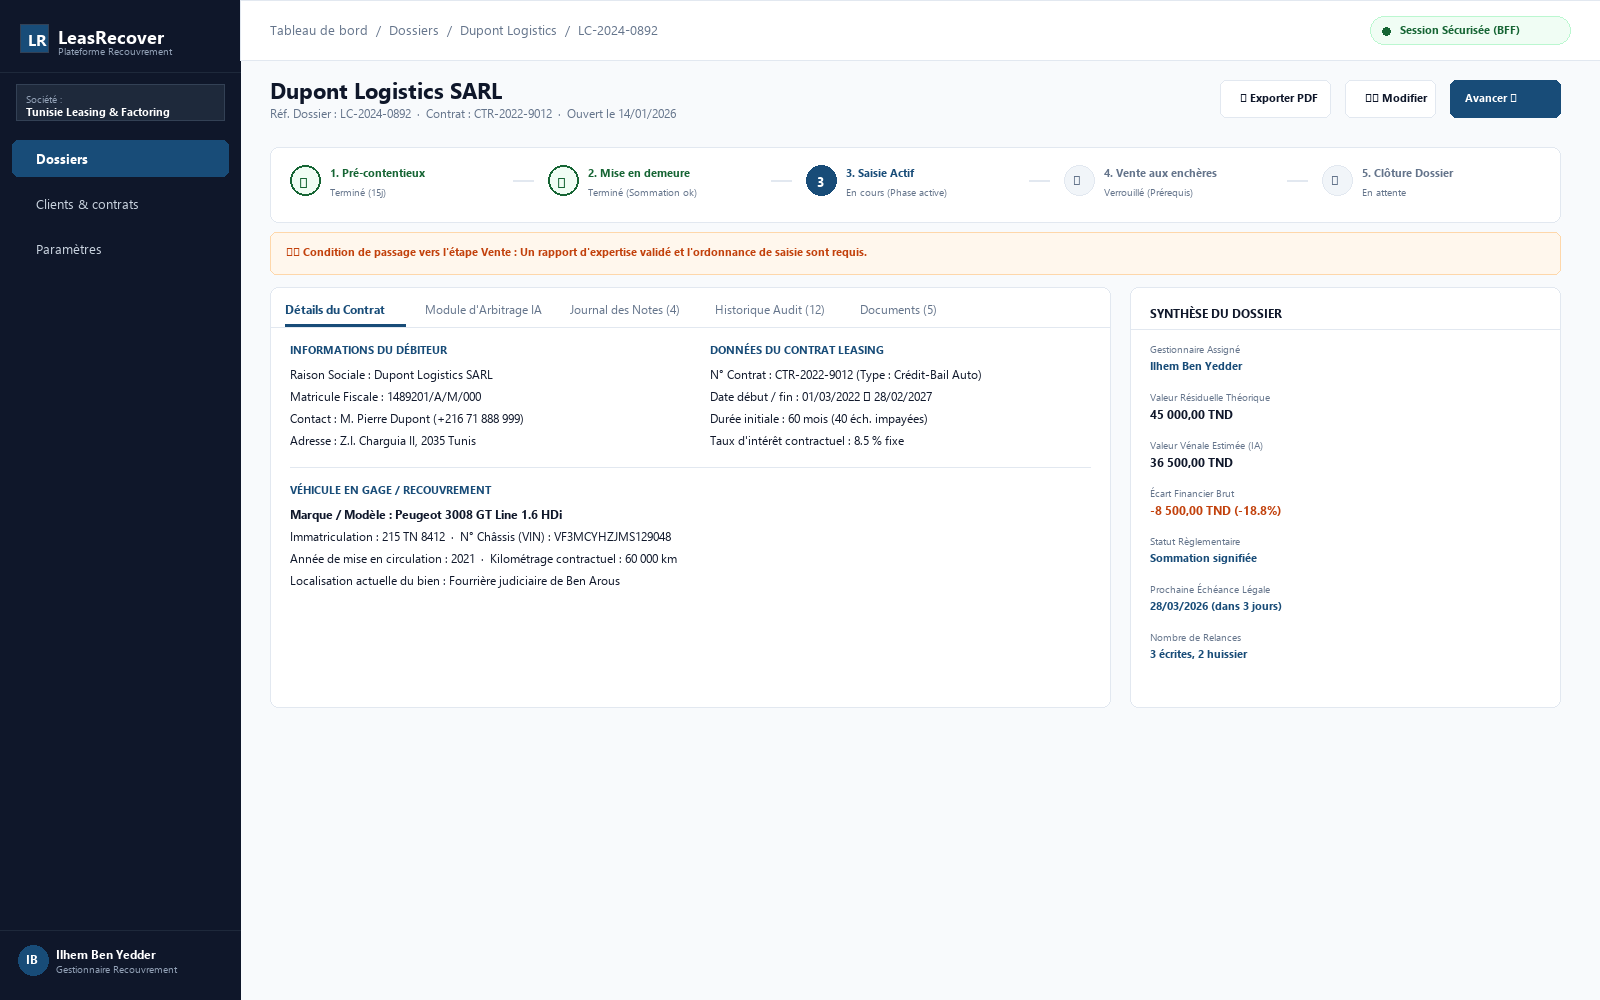
\includegraphics[width=0.95\textwidth,keepaspectratio]{images/screen_case_detail.png}
\caption{Fiche dossier interactive avec \textit{stepper} séquentiel et contrôle des prérequis}
\label{fig:screen_case_detail}
\end{figure}

%------------------------------------------------------------------------------
\subsection{Module d'Arbitrage et de Confrontation Financière IA}
\label{subsec:screen_ai_valuation}

Le module d'arbitrage (Figure~\ref{fig:screen_ai_valuation}) incarne la valeur ajoutée technologique de LeasRecover en automatisant la confrontation entre la valeur résiduelle contractuelle $\vr$ et la valeur vénale estimée par expertise $\ve$ :
\begin{itemize}
    \item \textbf{Carte d'Évaluation Financière (\textit{ValuationCard}) :} Affiche en format grand angle l'écart net calculé $\Delta = \ve - \vr$ (par exemple $-8\,500{,}00$~TND, soit $-18{,}89\,\%$).
    \item \textbf{Indicateur de Fiabilité Tripartite :} Attribution dynamique d'un badge visuel basé sur les seuils de tolérance configurés par l'institution :
    \begin{itemize}
        \item \textcolor{accentgreen}{\textbf{Fiable (Vert)}} : Écart faible ($|\Delta| < 10\,\%$), autorisant un passage rapide en vente aux enchères.
        \item \textcolor{accentorange}{\textbf{Écart Modéré (Orange)}} : Écart compris entre $10\,\%$ et $20\,\%$, nécessitant un arbitrage humain éclairé sur la mise à prix.
        \item \textcolor{accentred}{\textbf{Risque Critique (Rouge)}} : Écart supérieur à $20\,\%$, déclenchant une alerte majeure de dépréciation d'actif et une proposition de contre-expertise.
    \end{itemize}
    \item \textbf{Traçabilité et Provenance des Données Extraites :} Restitution transparente des données capturées par le modèle d'extraction (marque, modèle, année de mise en circulation, kilométrage certifié et estimation des frais de remise en état) avec lien d'accès direct au document PDF original.
    \item \textbf{Pipeline d'Ingestion Asynchrone en Temps Réel :} Feedback visuel étape par étape (\textit{Server-Sent Events}) informant le gestionnaire de l'état d'analyse du document (ingestion OCR, extraction NLP, rapprochement financier).
\end{itemize}

\begin{figure}[H]
\centering
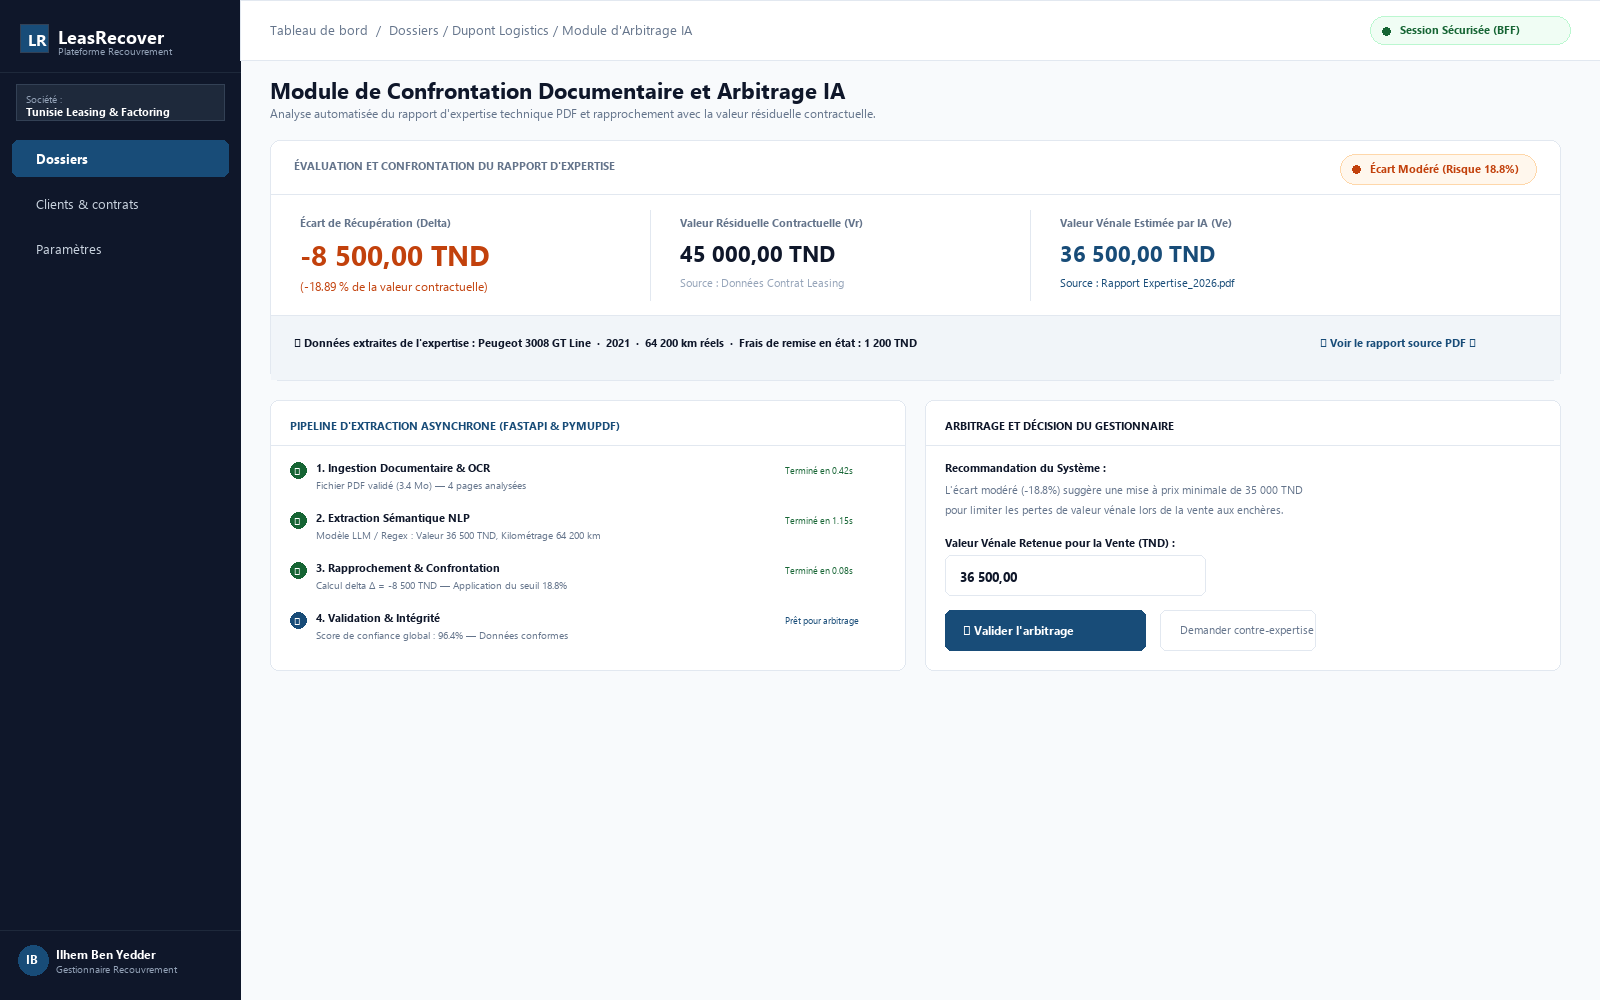
\includegraphics[width=0.95\textwidth,keepaspectratio]{images/screen_ai_valuation.png}
\caption{Module d'arbitrage financier et confrontation de l'expertise IA}
\label{fig:screen_ai_valuation}
\end{figure}

%------------------------------------------------------------------------------
\subsection{Gestion du Référentiel Métier du Leasing (Clients, Contrats et Actifs)}
\label{subsec:screen_leasing}

L'écran du référentiel métier (Figure~\ref{fig:screen_leasing}) assure la gouvernance des données de base de la société de crédit-bail :
\begin{itemize}
    \item \textbf{Répertoire Unifié des Débiteurs et Contrats :} Consultation à double niveau des entreprises clientes et de l'ensemble de leurs financements en cours.
    \item \textbf{Tiroir Latéral de Consultation (\textit{Side Sheet}) :} L'ouverture d'un client ou d'un contrat s'opère via un panneau coulissant à droite de l'écran, évitant la perte de repères visuels causée par les modales empilées traditionnelles.
    \item \textbf{Filiation Contractuelle et Matérielle :} Chaque contrat présente de manière exhaustive le véhicule gagé (numéro de châssis VIN, immatriculation, localisation physique en fourrière ou chez le débiteur) et le lien direct vers le dossier contentieux associé.
\end{itemize}

\begin{figure}[H]
\centering
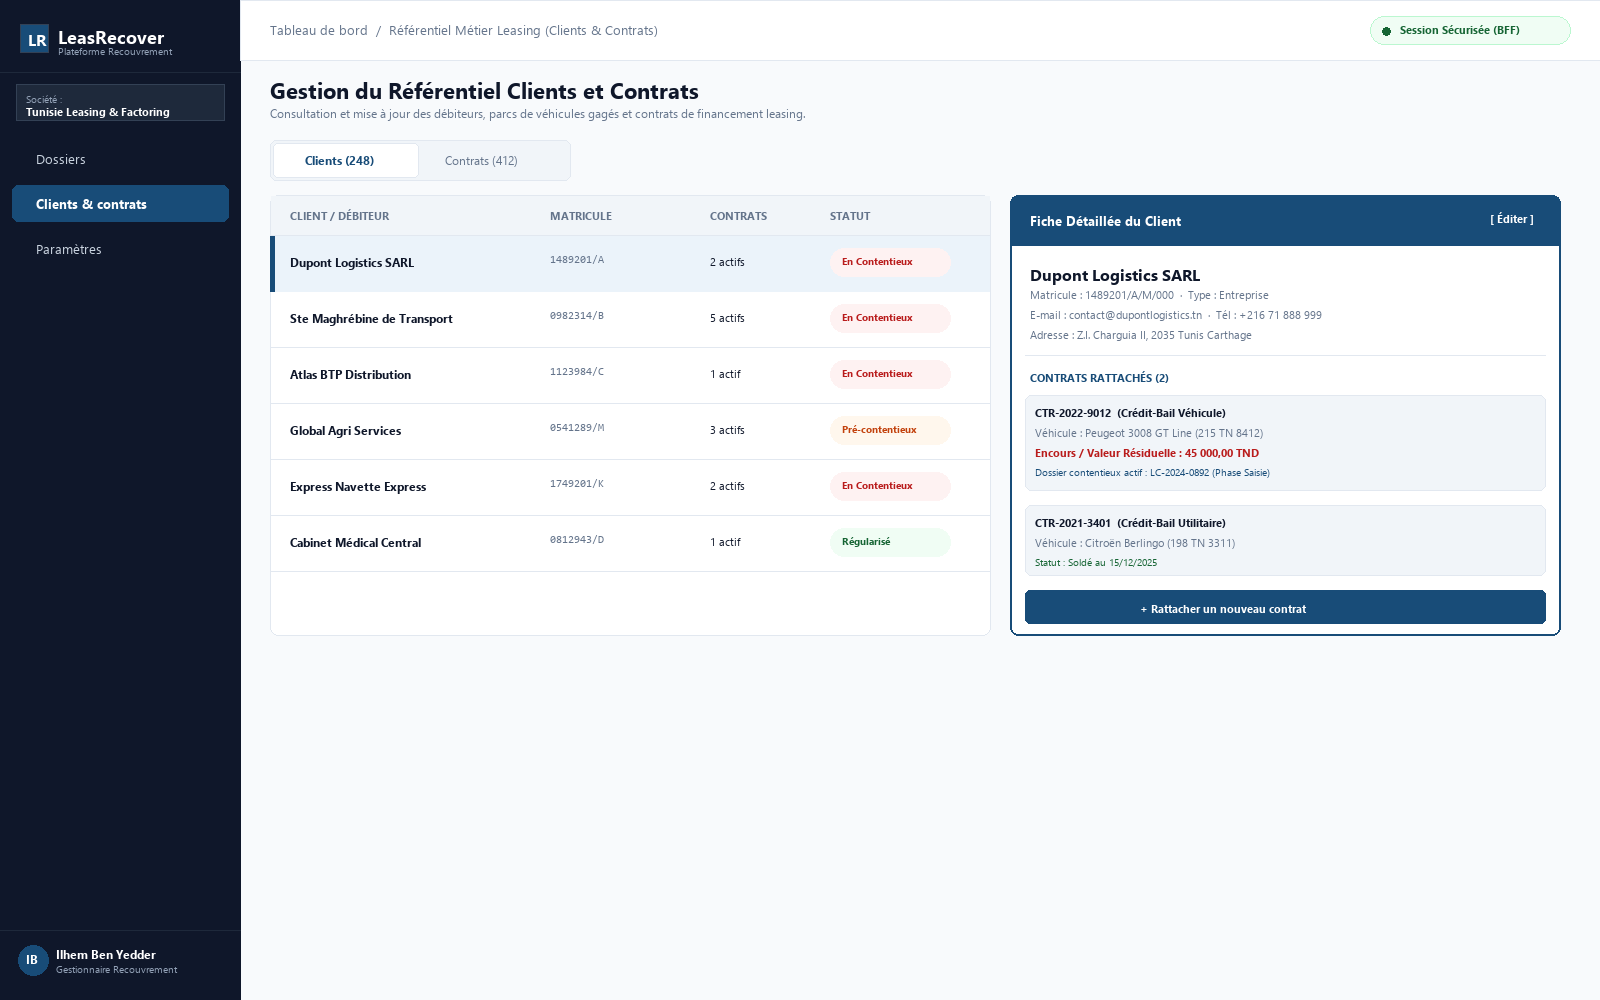
\includegraphics[width=0.95\textwidth,keepaspectratio]{images/screen_leasing.png}
\caption{Référentiel métier des contreparties et des actifs automobiles en crédit-bail}
\label{fig:screen_leasing}
\end{figure}

%------------------------------------------------------------------------------
\subsection{Paramétrage Institutionnel et Règles de Conformité}
\label{subsec:screen_admin_settings}

L'écran de configuration institutionnelle (Figure~\ref{fig:screen_admin_settings}) permet aux responsables conformité et directeurs de recouvrement de calibrer le comportement du système sans modification de code :
\begin{itemize}
    \item \textbf{Délais Légaux par Phase :} Définition des durées maximales autorisées pour chaque phase (par exemple 15 jours en pré-contentieux, 8 jours pour la mise en demeure, 30 jours pour la saisie conservatoire), avec paramétrage du délai d'alerte anticipée (48h avant l'échéance).
    \item \textbf{Seuil d'Alerte de Dormance :} Fixation du nombre maximal de jours d'inactivité tolérés sur un dossier avant notification automatique au superviseur.
    \item \textbf{Calibrage des Seuils IA avec Prévisualisation en Direct :} Ajustement en pourcentage des bornes de criticité pour l'analyse des rapports d'expertise, accompagné d'une prévisualisation dynamique des règles de décision appliquées.
\end{itemize}

\begin{figure}[H]
\centering
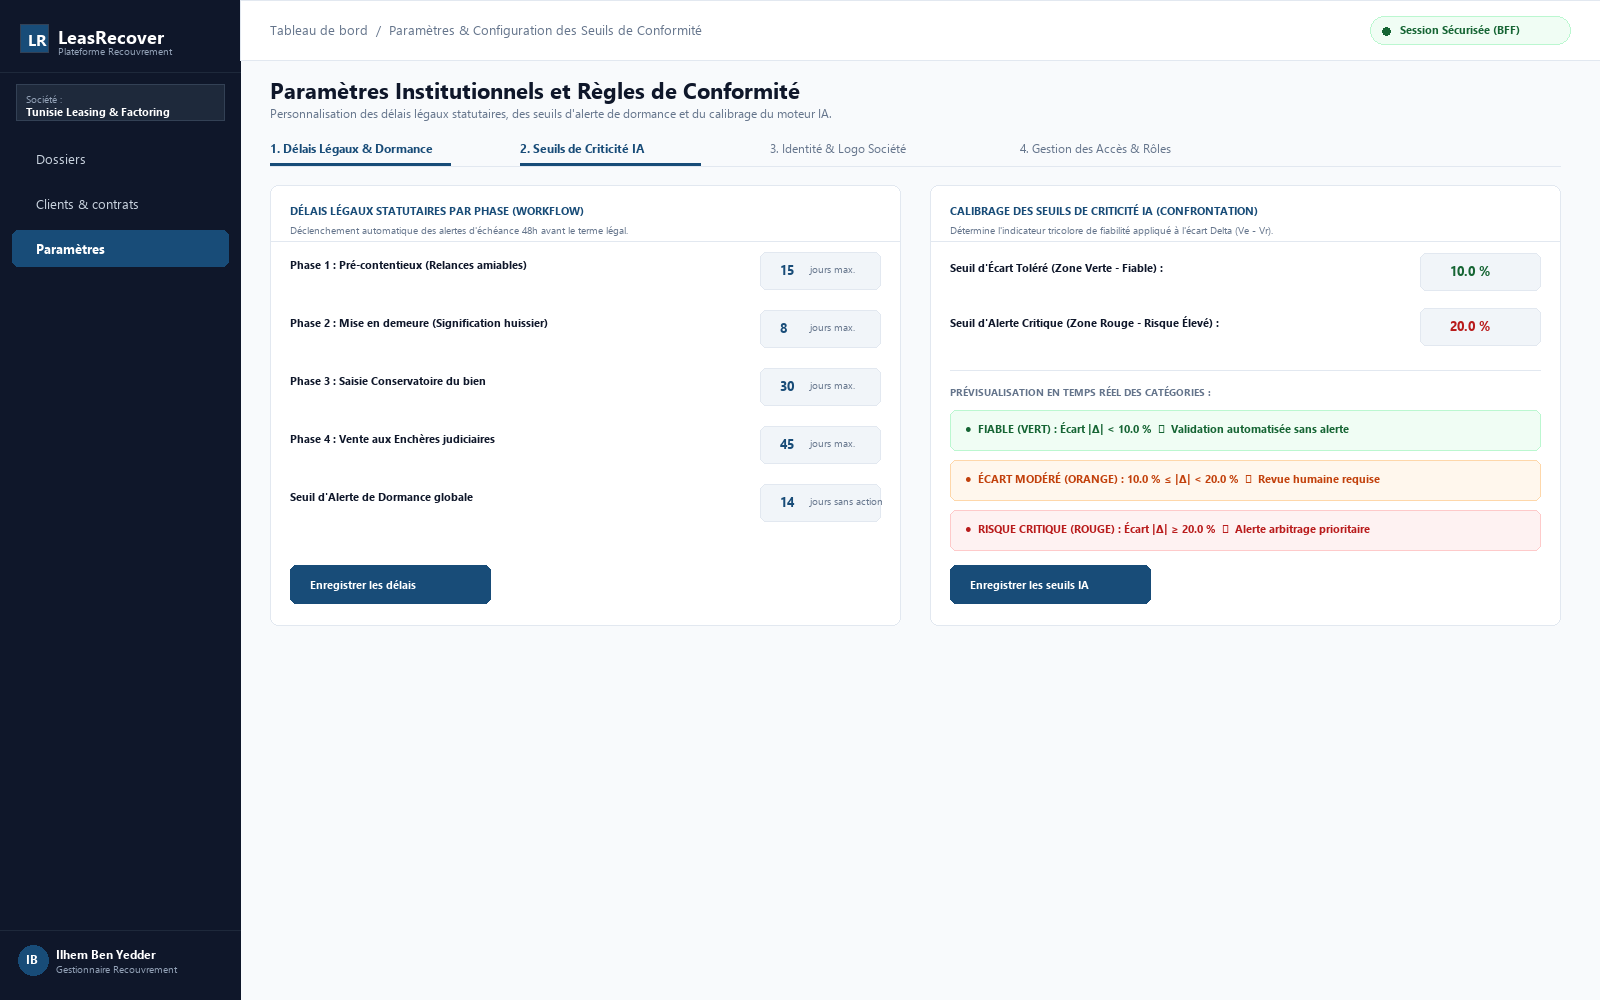
\includegraphics[width=0.95\textwidth,keepaspectratio]{images/screen_admin_settings.png}
\caption{Interface de paramétrage des délais légaux et des seuils de criticité IA}
\label{fig:screen_admin_settings}
\end{figure}

\section{Stratégie de Tests et Validation Expérimentale}

\subsection{Pyramide de Tests Réalisée}

La conformité et la sécurité du système ont été validées selon une approche multi-niveaux :
\begin{itemize}
    \item \textbf{Tests Unitaires (Spring Boot \& FastAPI) :} Validation des algorithmes de calcul financier, des règles de transition d'états et de l'étanchéité des parseurs PDF.
    \item \textbf{Tests d'Intégration API :} Vérification des points de terminaison REST, du cycle de vie des sessions BFF et de la persistance sous PostgreSQL 18.
    \item \textbf{Tests d'Étanchéité Multi-Tenant :} Simulation d'attaques d'injection et de requêtes inter-tenants pour vérifier l'absence totale de fuite de données (\textit{Zero Data Leakage}).
\end{itemize}

\subsection{Résultats de Validation}

Le tableau~\ref{tab:resultats_tests} synthétise les résultats obtenus lors de la campagne de qualification.

\begin{table}[H]
\centering
\small
\caption{Matrice de validation et résultats des cas de tests clés}
\label{tab:resultats_tests}
\begin{tabularx}{\textwidth}{@{}L{3.2cm} Y L{1.5cm} L{2.6cm}@{}}
\toprule
\textbf{Référence Test} & \textbf{Objectif et Scénario Validé} & \textbf{Statut} & \textbf{Taux de Succès} \\
\midrule
\textbf{TC-SEC-01} & Authentification BFF, session HttpOnly et isolation tenant & Succès & 100\% conforme \\
\addlinespace
\textbf{TC-TENANT-02} & Tentative de lecture de données d'un autre tenant (schéma SQL) & Succès & Bloqué (HTTP 403) \\
\addlinespace
\textbf{TC-WORKFLOW-03} & Progression séquentielle stricte des 5 phases juridiques & Succès & 100\% règles respectées \\
\addlinespace
\textbf{TC-AI-04} & Extraction IA sur un jeu de 50 rapports d'expertise réels & Succès & Précision $\ge 94.2\%$ \\
\addlinespace
\textbf{TC-FINANCE-05} & Calcul exact de l'écart $\Delta = |\ve - \vr|$ et catégorisation & Succès & 100\% au centime près \\
\bottomrule
\end{tabularx}
\end{table}

\section{Conclusion}

La phase de réalisation a permis de concrétiser les exigences techniques et fonctionnelles de \projectShortTitle. L'intégration harmonieuse de Next.js, Spring Boot et FastAPI, alliée à la rigueur de l'isolation multi-tenant et à la précision du pipeline d'intelligence artificielle, aboutit à une solution industrielle performante et directement opérationnelle.
